The \textit{User Management} module is responsible for maintaining demographic information
about the registered users of the system, including the Authority levels of each
user.



\subsection{Scope}
The scope for the users module is shown in Figure \ref{Users Scope}
\begin{figure}[H]
  \begin{center}
  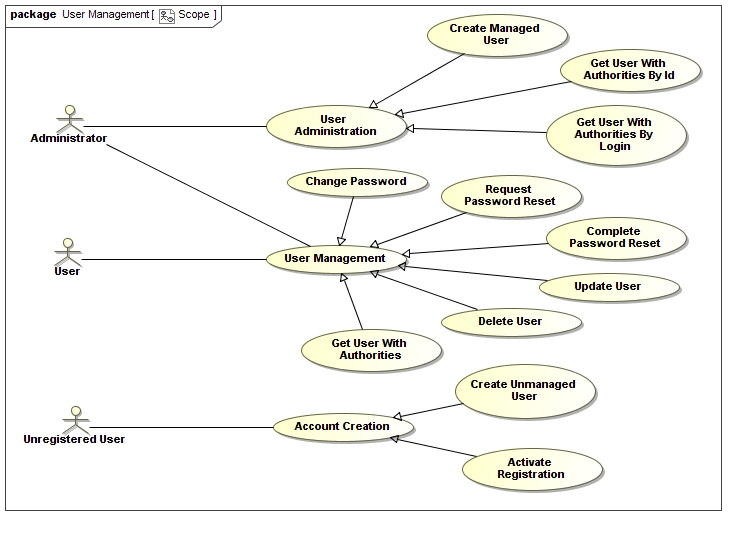
\includegraphics[scale=0.4]{../Diagrams and Charts/User Management/Scope.jpg}
  \caption{Users Scope}
  \end{center}
  \label{Users Scope}
\end{figure}
The scope of the users module include:
\begin{itemize}
	\item Administrator users can add and remove Regular Users
	\item Any person who wants use the benchmarking service can register
	to the system and become a user. They can then also edit
	their profile.
\end{itemize}



\subsection{Domain Model}
The domain model for the users module is shown in Figure \ref{Users Domain Model}
\begin{figure}[H]
  \begin{center}
  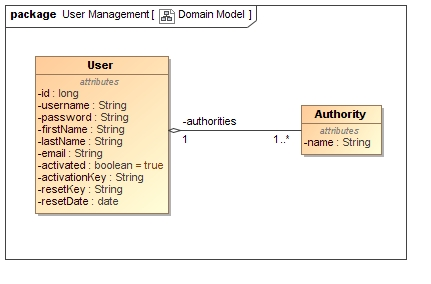
\includegraphics[scale=0.4]{../Diagrams and Charts/User Management/Domain Model.jpg}
  \caption{Users Domain Model}
  \end{center}
  \label{Users Domain Model}
\end{figure}

There are 2 main types of users who are at different authority levels. 
\textit{Administrator} users will have the permissions needed to manage the 
website, manage regular users and do certain administrative duties on the
system.

\textit{Users} can be registered by anyone who wants to use the benchmarking 
service. These users will be able to conduct benchmarks but will not be able to
preform any administrative duties on the system.



\subsection{Activate Registration}
The \textit{Activate Registration} use case is concerned with activating the
account of a user created by the \textit{Create Unmanaged User} service.

\subsubsection{Services Contract}
The service contract for activating a user account is shown in 
Figure \ref{fig:activateRegistrationServiceContract}.
\begin{figure}[H]
	\begin{center}
		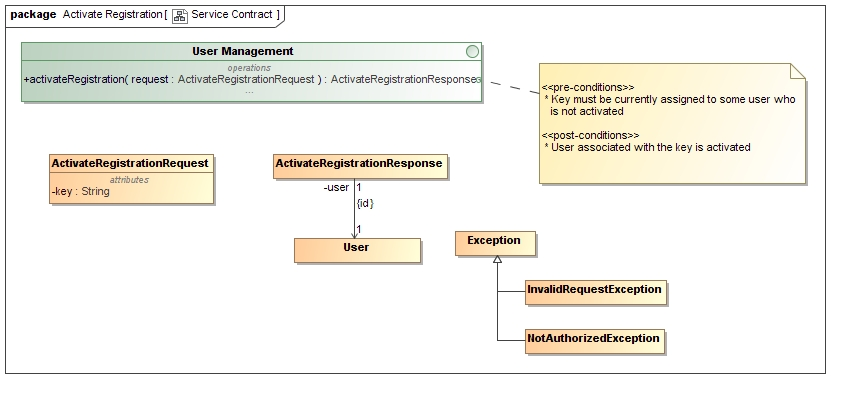
\includegraphics[scale=0.4]{../Diagrams and Charts/User Management/Activate Registration Service Contract.jpg}
		\caption{Activate Registration Service Contract}
		\label{fig:activateRegistrationServiceContract}
	\end{center}
\end{figure}
 


\subsection{Change Password}
The \textit{Change Password} use case is concerned with allowing the currently
logged-in user to change their password.

\subsubsection{Services Contract}
The service contract for removing a registered monitor node from the back end 
system is shown in Figure \ref{fig:removeNodeServiceContract}.
\begin{figure}[H]
  \begin{center}
  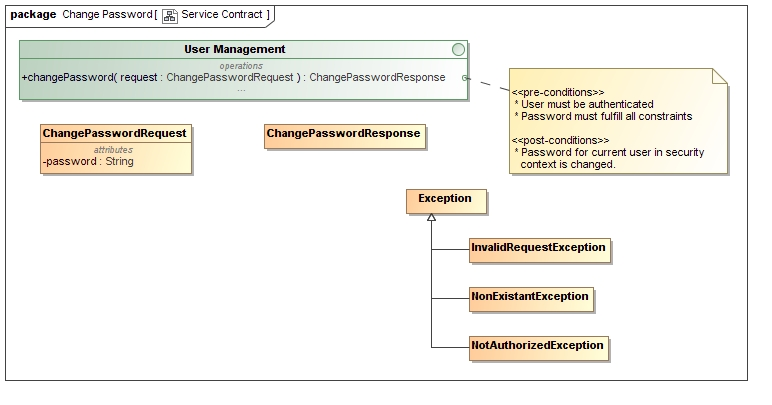
\includegraphics[scale=0.4]{../Diagrams and Charts/User Management/Change Password Service Contract.jpg}
  \caption{Change Password Service Contract}
  \label{fig:changePasswordServicesContract}
  \end{center}
\end{figure}



\subsection{Complete Password Reset}
The \textit{Complete Password Reset} use case is concerned with setting the
new password of a lost account. This is the final step to complete on an account
after the \textit{Request Password Reset} service has been called first on the
lost account.

\subsubsection{Services Contract}
The service contract for removing a registered monitor node from the back end 
system is shown in Figure \ref{fig:removeNodeServiceContract}.
\begin{figure}[H]
  \begin{center}
  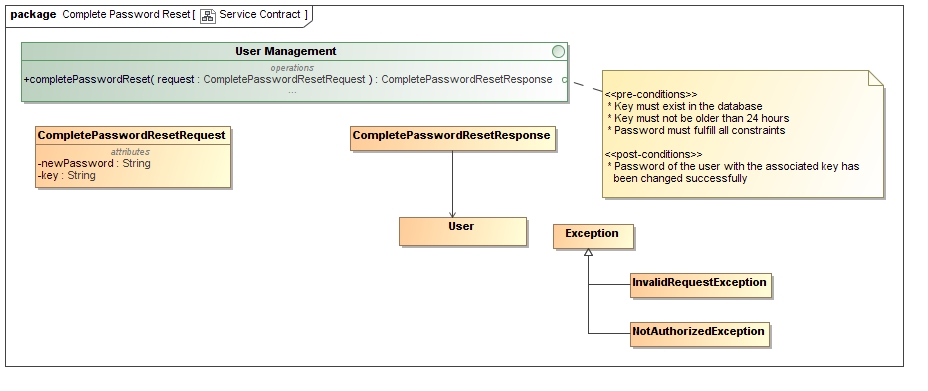
\includegraphics[scale=0.4]{../Diagrams and Charts/User Management/Complete Password Reset Service Contract.jpg}
  \caption{Complete Password Reset Service Contract}
  \label{fig:completePasswordResetServicesContract}
  \end{center}  
\end{figure}



\subsection{Create Managed User}
The \textit{Create Managed User} use case is concerned with allowing an
administrator to create a user account deferring the selection of password to the
final user.

\subsubsection{Services Contract}
The service contract for removing a registered monitor node from the back end 
system is shown in Figure \ref{fig:createManagedUserServicesContract}.
\begin{figure}[H]
	\begin{center}
		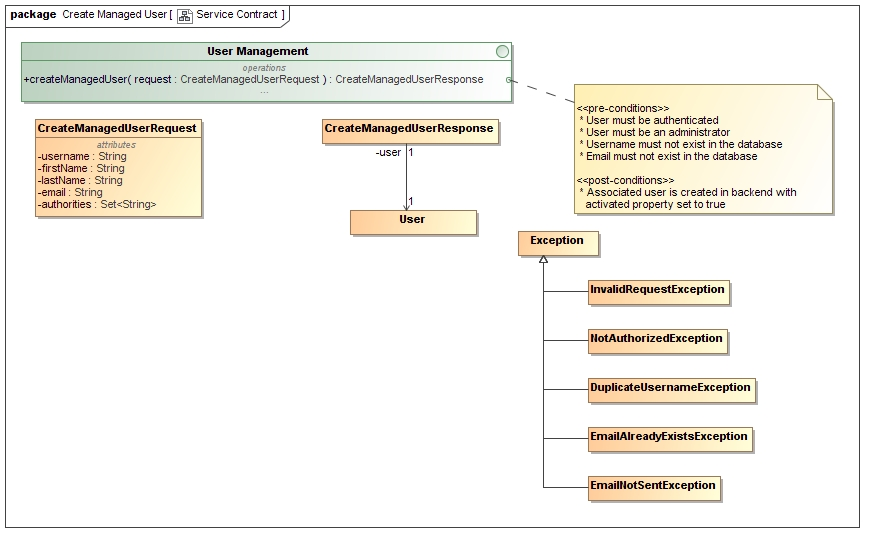
\includegraphics[scale=0.4]{../Diagrams and Charts/User Management/Create Managed User Service Contract.jpg}
		\caption{Create Managed User Service Contract}
		\label{fig:createManagedUserServicesContract}
	\end{center}
\end{figure}



\subsection{Create Unmanaged User}
The \textit{Create Unmanaged User} use case is concerned with allowing a user to
create for themselves an account on the benchmark system, with a default role
of \textit{User}.

\subsubsection{Services Contract}
The service contract for removing a registered monitor node from the back end 
system is shown in Figure \ref{fig:CreateUnmanagedUserServicesContract}.
\begin{figure}[H]
  \begin{center}
  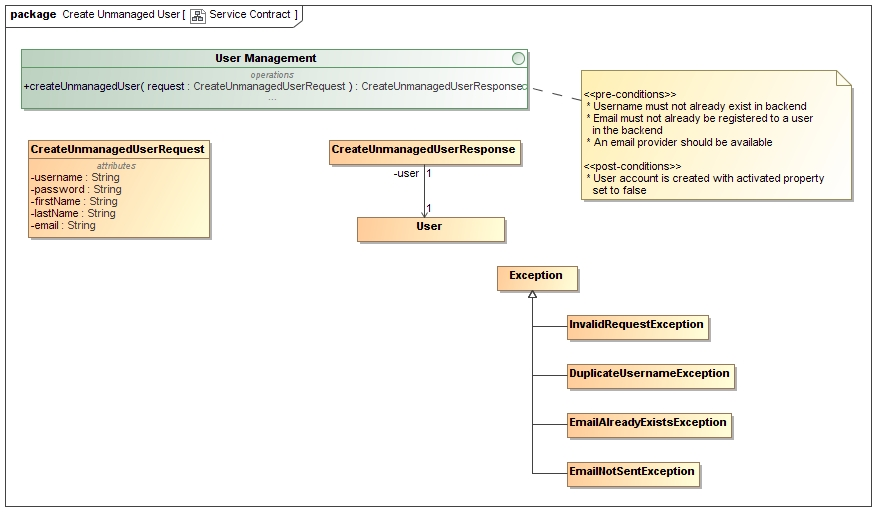
\includegraphics[scale=0.4]{../Diagrams and Charts/User Management/Create Unmanaged User Service Contract.jpg}
  \caption{Create Unmanaged User Service Contract}
  \label{fig:CreateUnmanagedUserServicesContract}
  \end{center}  
\end{figure}

\subsubsection{Process Design}
Refer to figure \ref{fig:CreateUnmanagedUserProcessDesign} on the process flow to
create a new unmanaged user account, i.e. the end user creates there own account.
Note that the Get user With Authorities service is used to confirm if another
user with that same username already exists in the system, if so an DuplicateUsernameException
is raised. Next the Create Unmanaged User user is responsible for confirming that
no account is already associated with the email address passed in with the request
object. If email address is already associated with an account a EmailAlreadyExistsException
is raised. After the account has been created a notification will be sent to the
user. If email could not be sent to the user, a EmailNotSentException is raised.
\begin{figure}[H]
  \begin{center}
  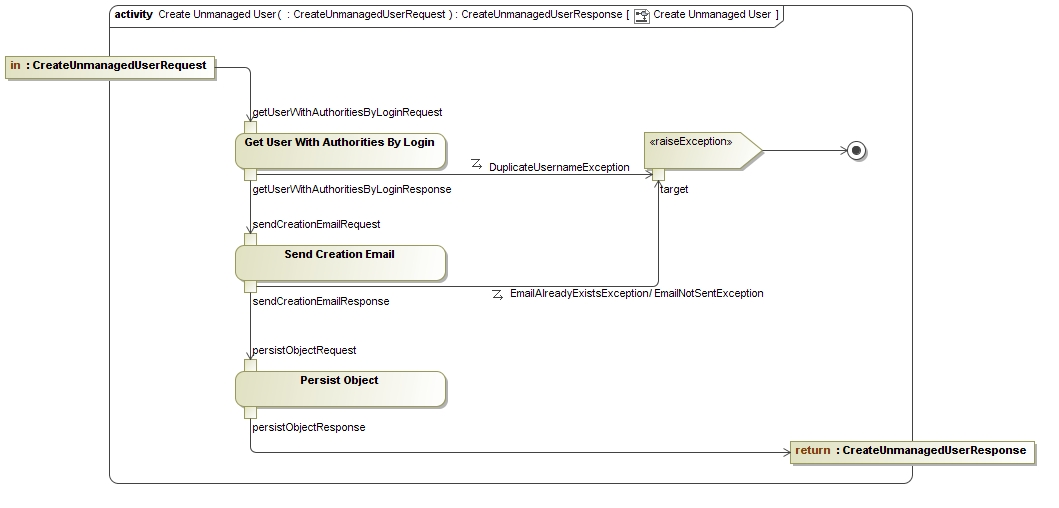
\includegraphics[scale=0.38]{../Diagrams and Charts/User Management/Create Unmanaged User Process Design.jpg}
  \caption{Create Unmanaged User Process Design}
  \label{fig:CreateUnmanagedUserProcessDesign}
  \end{center}
\end{figure}



\subsection{Delete User}
The \textit{Delete User} use case is concerned removing a user from the back end
system.

\subsubsection{Services Contract}
The service contract for removing a registered monitor node from the back end 
system is shown in Figure \ref{fig:deleteUserServicesContract}.
\begin{figure}[H]
	\begin{center}
		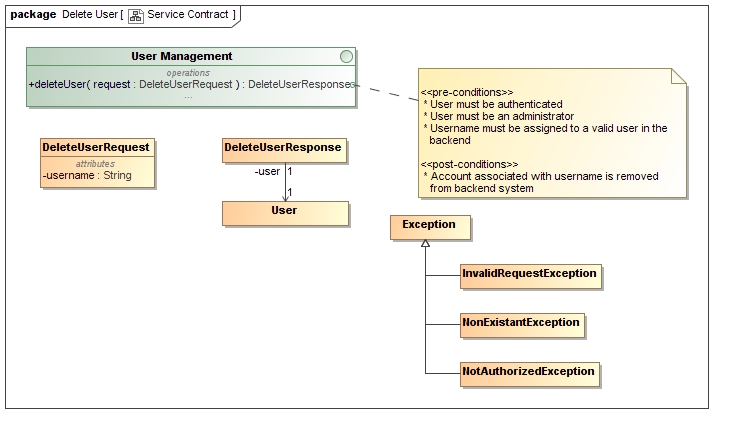
\includegraphics[scale=0.4]{../Diagrams and Charts/User Management/Delete User Service Contract.jpg}
		\caption{Delete User Service Contract}
		\label{fig:deleteUserServicesContract}
	\end{center}
\end{figure}



\subsection{Get User With Authorities}
The \textit{Get User With Authorities} use case is concerned with retrieving the
current user with associated roles from the current security context.

\subsubsection{Services Contract}
The service contract for removing a registered monitor node from the back end 
system is shown in Figure \ref{fig:getUserWithAuthoritiesServicesContract}.
\begin{figure}[H]
	\begin{center}
		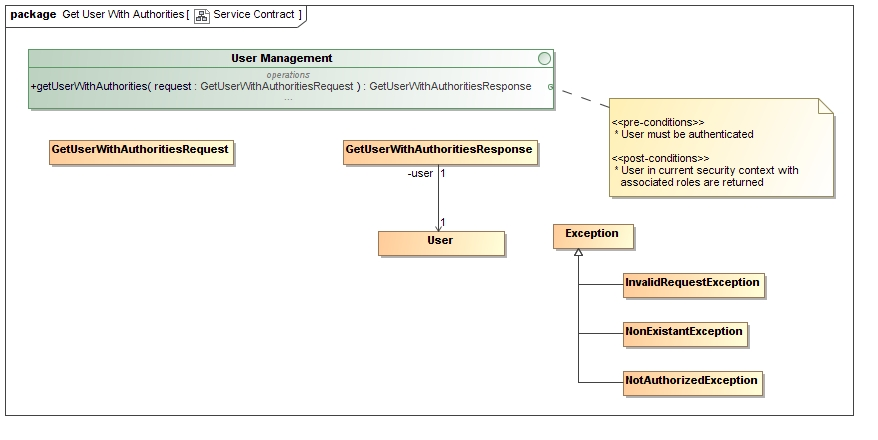
\includegraphics[scale=0.4]{../Diagrams and Charts/User Management/Get User With Authorities Service Contract.jpg}
		\caption{Get User With Authorities Service Contract}
		\label{fig:getUserWithAuthoritiesServicesContract}
	\end{center}
\end{figure}



\subsection{Get User With Authorities By Login}
The \textit{Get User With Authorities By Login} use case is concerned with
retrieving a specified user with there associated roles from the back end.

\subsubsection{Services Contract}
The service contract for removing a registered monitor node from the back end 
system is shown in Figure \ref{fig:getUserWithAuthoritiesByLoginServicesContract}.
\begin{figure}[H]
	\begin{center}
		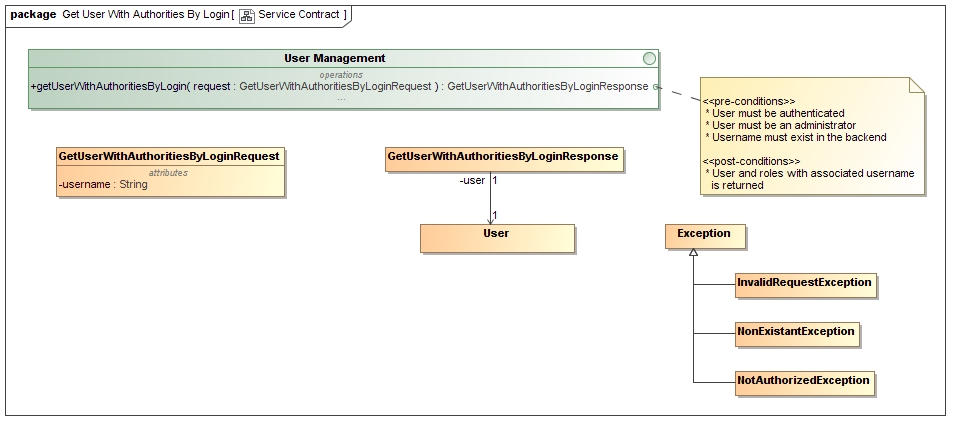
\includegraphics[scale=0.4]{../Diagrams and Charts/User Management/Get User With Authorities By Login Service Contract.jpg}
		\caption{Get User With Authorities By Login Service Contract}
		\label{fig:getUserWithAuthoritiesByLoginServicesContract}
	\end{center}
\end{figure}



\subsection{Request Password Reset}
The \textit{Request Password Reset} use case is concerned with allowing a user
to retrieve a lost account. This is the first step in account retrieval, with the
second and final step being the \textit{Complete Password Reset} service.

\subsubsection{Services Contract}
The service contract for removing a registered monitor node from the back end 
system is shown in Figure \ref{fig:requestPasswordResetServicesContract}.
\begin{figure}[H]
  \begin{center}
  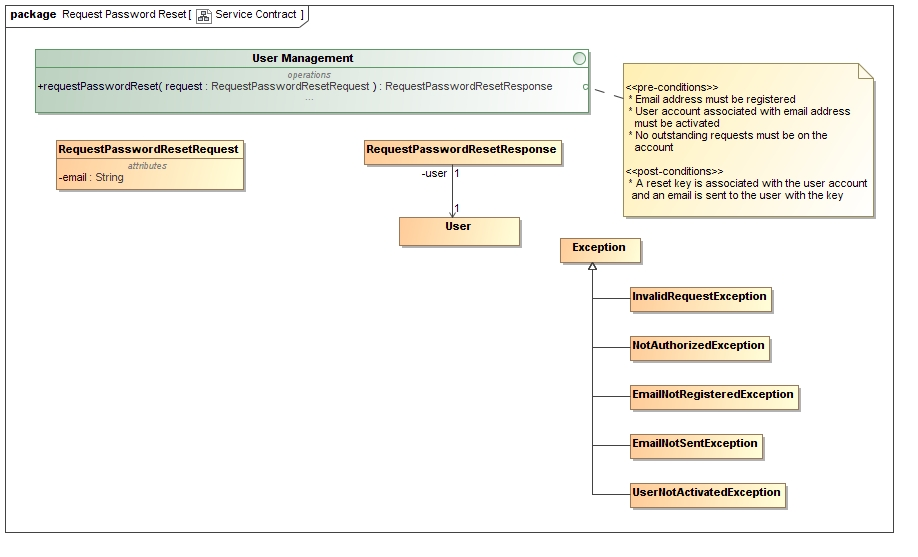
\includegraphics[scale=0.4]{../Diagrams and Charts/User Management/Request Password Reset Service Contract.jpg}
  \caption{Request Password Reset Service Contract}
  \label{fig:requestPasswordResetServicesContract}
  \end{center}  
\end{figure}



\subsection{Update User}
The \textit{Update User} use case is concerned with allowing the currently
logged-in user to update their associated profile data. Important to note is 
that the user is not able to update their username.
 
\subsubsection{Services Contract}
The service contract for removing a registered monitor node from the back end 
system is shown in Figure \ref{fig:updateUserServicesContract}.
\begin{figure}[H]
	\begin{center}
		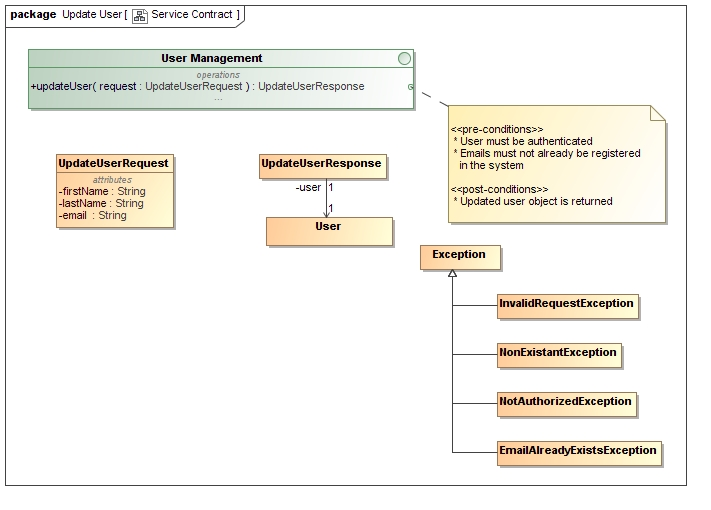
\includegraphics[scale=0.4]{../Diagrams and Charts/User Management/Update User Service Contract.jpg}
		\caption{Update User Service Contract}
		\label{fig:updateUserServicesContract}
	\end{center}
\end{figure}

\subsubsection{Functional Requirements}
The lower level services required by the create experiment service to 
either check the pre-conditions or address the post-conditions is shown in
Figure \ref{fig:updateUserFunctionalRequirements}.
\begin{figure}[H]
	\begin{center}
		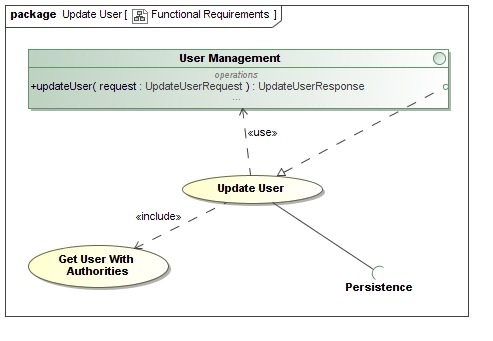
\includegraphics[scale=0.4]{../Diagrams and Charts/User Management/Update User Functional Requirements.jpg}
		\caption{Update User Functional Requirements}
		\label{fig:updateUserFunctionalRequirements}
	\end{center}	
\end{figure}
